\documentclass[a4paper,12pt]{article}

\usepackage{cmap}
\usepackage{mathtext}
\usepackage[T2A]{fontenc}
\usepackage[utf8]{inputenc}
\usepackage[english,russian]{babel}
\usepackage{indentfirst}
\frenchspacing


\usepackage{amsmath,amsfonts,amssymb,amsthm,mathtools} % AMS
\usepackage{icomma}

\DeclareMathOperator{\sgn}{\mathop{sgn}}

\newcommand*{\hm}[1]{#1\nobreak\discretionary{}
{\hbox{$\mathsurround=0pt #1$}}{}}

\usepackage{graphicx}
\graphicspath{{images/}{images2/}}
\setlength\fboxsep{3pt}
\setlength\fboxrule{1pt}
\usepackage{wrapfig}

\usepackage{array,tabularx,tabulary,booktabs}
\usepackage{longtable}
\usepackage{multirow}

\theoremstyle{plain}
\newtheorem{theorem}{Теорема}[section]
\newtheorem{proposition}[theorem]{Утверждение}
 
\theoremstyle{definition}
\newtheorem{corollary}{Следствие}[theorem]
\newtheorem{problem}{Задача}[section]
 
\theoremstyle{remark}
\newtheorem*{nonum}{Решение}

\usepackage{etoolbox}


\usepackage{extsizes}
\usepackage{geometry}
	\geometry{top=25mm}
	\geometry{bottom=35mm}
	\geometry{left=35mm}
	\geometry{right=20mm}

\usepackage{setspace}

\usepackage{lastpage}

\usepackage{soul}

\usepackage{hyperref}
\usepackage[usenames,dvipsnames,svgnames,table,rgb]{xcolor}
\hypersetup{
    unicode=true,
    pdftitle={Заголовок},
    pdfauthor={Автор},
    pdfsubject={Тема},
    pdfcreator={Создатель},
    pdfproducer={Производитель},
    pdfkeywords={keyword1} {key2} {key3},
    colorlinks=true,
    linkcolor=red,
    citecolor=black,
    filecolor=magenta,
    urlcolor=cyan
}

\usepackage{csquotes} % Еще инструменты для ссылок

%\usepackage[style=authoryear,maxcitenames=2,backend=biber,sorting=nty]{biblatex}

\usepackage{multicol} % Несколько колонок

\usepackage{tikz} % Работа с графикой
\usepackage{pgfplots}
\usepackage{pgfplotstable}

\newcommand{\nl}{\\ \indent}

%\author{}
%\title{}
%\date{}

\begin{document} % конец преамбулы, начало документа
\tableofcontents
\newpage
\section{Математическая постановка задачи}
\subsection{Постановка задачи}
В экспериментальных исследованиях результатом 
измерения является конечный набор значений
$\pmb{\xi} = (\xi_1, \ldots, \xi_N)$,
где $\xi_i$ -- наклонное содержание
$\text{NO}_2$ для зинитного угла направления
визирования $z_i$.
По набору этих значений требуется оценить значения вертикального
распределения $\text{NO}_2$ $n(h)$ в заданном наборе точек
области определения.
\nl
В задаче восстановления $\text{NO}_2$ результат измерения
имеет вид:
\begin{equation}
\xi_i = 
\int_{0}^{H}m(z_i, h)n(h)dh + \nu_i =
\sum\limits_{j=1}^{M}m(z_i, h_j) n(h_j) \triangle h
+ \nu_i = (a_i, n) + \nu_i
\end{equation}
где $a_i$ -- послойная воздушная масса,
которая рассчитывается из модели переноса излучения.
Она связывает наклонное содержание
$\text{NO}_2$ $\pmb{\xi}$
с вертикальным распределением концентраций $n(h)$.
\nl
Схему измерений можно представить в виде:
\begin{equation}
\pmb\xi = A \pmb{n} + \pmb{\nu}
\end{equation}
На основании измерения вектора
$\pmb\xi = (\xi_1, \ldots, \xi_N)$
требуется оценить значение вектора
$Un \in \mathbb{R}^N$, 
где $U: \mathbb{R}^N \rightarrow \mathbb{R}^N$ --
оператор, которому сопоставляется матрица с учётом 
априорной информации о значениях координат вектора $\pmb{n}$.
\subsection{Обратные задачи}
Рассмотрим неизвестный сигнал 
$f \in \mathcal{L}^2(\mathbb{R}^d)$ и предположим, 
что последний проверяется каким-либо сенсорным устройством, 
что приводит к вектору данных 
$\textbf{y} = [y_1, \ldots, y_L]$ из $L$ измерения. 
Восстановление $f$ из вектора данных $\textbf{y}$ 
называется обратной задачей.
\nl
Следующие допущения являются стандартными:
\begin{itemize}
\item Чтобы учесть неточности датчиков предполагается, 
что вектор данных $\textbf{u}$ это результат 
случайного вектора 
$\textbf{Y} = [Y_1, \ldots , Y_L] =
\left[ 
\langle f, \phi_1 \rangle,
\ldots ,
\langle f, \phi_L \rangle
\right]$, 
колеблющийся в соответствии с некоторым распределением шума. 
Записи $\mathbb{E}[\textbf{Y}] = \widetilde{\textbf{y}}$ 
называются идеальными измерениями(измерения, которые были бы получены в отсутствие шума).
\item Измерения предполагаются несмещенными и линейными,
т.е.
$\mathbb{E}[\textbf{Y}] = \Phi^{*}f$, 
для некоторых функционалов выборки 
$\{ \phi_1, \ldots , \phi_L \} 
\subset \mathcal{L}^2(\mathbb{R}^d)$ 
моделирующих систему сбора данных.
\end{itemize}
\subsection{Некорректность обратных задач}
Для решения обратной задачи можно аппроксимировать 
среднее $\mathbb{E}[Y]$ по его одновыборочной эмпирической 
оценке $\textbf{y}$ и решить линейную задачу:
\begin{equation}
\label{eq_1}
\textbf{y} = \textbf{G} \alpha
\end{equation}
К сожалению, такие задачи в целом некорректны:
\begin{itemize}
\item \textbf{Решений может не быть}. 
Если $\textbf{G}$ не сюръективен,
$\mathcal{R}(\textbf{G}) \subseteq \mathbb{R}^L$. 
Следовательно, зашумленный вектор данных $\textbf{y}$ 
не гарантируется принадлежность к $\mathcal{R}(\mathbb{G})$.
\item \textbf{Может существовать более одного решения}. 
Если $L < N$ действительно (или, в более общем смысле, если 
$\textbf{G}$ не инъективен), 
$\mathcal{N}(\textbf{G}) \neq \{ \textbf{0} \}$. 
Следовательно, если $\alpha^{*}$ является решением 
\eqref{eq_1}, тогда $\alpha^{*} + \beta$ также является решением
$\forall \beta \in \mathcal{N}(\textbf{G})$:
\[
\textbf{G}(\alpha^{*} + \beta) =
\textbf{G} \alpha^{*} + \textbf{G} \beta =
\textbf{G} \alpha^{*} = \textbf{y}
\]
\item \textbf{Решения могут быть численно неустойчивыми}.
Если $\textbf{G}$ например, сюръективно, то
$\textbf{G}^{\dagger} = 
\textbf{G}^{T}(\textbf{G} \textbf{G}^{T})^{-1}$
является правой инверсией $\textbf{G}$,
а также 
$\alpha^{*}(\textbf{y}) =
\textbf{G}^{T}(\textbf{G} \textbf{G}^{T})^{-1}$
является решением \eqref{eq_1}. 
У нас есть тогда
\[
||\alpha^{*}(\textbf{y})|| \leq
||\textbf{G}||_{2}
||(\textbf{G}^{T} \textbf{G})^{-1}||_2
||\textbf{y}||_2 =
\underbrace{
\dfrac{
\sqrt{\lambda_{\text{max}}(\textbf{G}^{T}\textbf{G}})
}{
\lambda_{\text{min}}(\textbf{G}^{T}\textbf{G})
}}_{\text{может быть очень большим}} 
||\textbf{y}||_2, \qquad 
\forall \textbf{y} \in \mathbb{R}^L.
\]
\end{itemize}
\subsection{Регуляризация обратных задач}
Линейная система \eqref{eq_1} не только некорректна, 
но и бессмысленна: точное совпадение измерений нежелательно, 
так как последние на практике искажаются инструментальными шумами.
\nl
Вместо этого более разумный подход состоит в решении 
обратной задачи с помощью штрафной задачи оптимизации, 
сопоставляя физические данные с априорными представлениями
аналитика о решении (например, гладкость, разреженность) 
с помощью терминов точности данных и регуляризации 
соответственно:
\[
\min_{\alpha \in \mathbb{R}^N}
F(\textbf{y}, \textbf{G} \alpha) +
\lambda \mathcal{R} (\alpha)
\]
Различные величины, участвующие в приведенном выше уравнении, 
можно интерпретировать следующим образом:
\begin{itemize}
\item 
$F: \mathbb{R}^L \times \mathbb{R}^L 
\rightarrow \mathbb{R}_{+} \cup \{ + \infty \}$
представляет собой функционал 
стоимости/верности данных/потери, 
измеряющий несоответствие между наблюдаемыми и 
прогнозируемыми измерениями $\textbf{y}$, 
а также $\textbf{G} \alpha$ соответственно.
\item 
$\mathcal{R}: \mathbb{R}^N 
\rightarrow \mathbb{R}_{+} \cup \{ + \infty \}$ является
функционалом регуляризации/штрафа,
отдающим предпочтение простым и хорошим решениям 
(обычно с конечным числом степеней свободы).
\item 
$\lambda > 0$ является параметром регуляризации/штрафа, 
который контролирует степень регуляризации, 
помещая функционал регуляризации и функционал 
стоимости в одинаковую шкалу.
\end{itemize}
\subsection{Выбор функционала потерь}
Функционал потерь можно выбрать как отрицательное 
логарифмическое правдоподобие данных $\textbf{y}$:
\[
F(\textbf{y}, \textbf{G} \alpha) =
- \ell(\alpha | \textbf{y}) =
- \log p_{Y_1, \ldots, Y_L}
(y_1, \ldots, y_L | \alpha).
\]
Когда распределение шума не известно полностью или 
вероятность слишком сложна, 
можно также использовать общие $\ell_p$ функционалы стоимости:
\[
F(\textbf{y}, \textbf{G} \alpha) =
||\textbf{y} - \textbf{G} \alpha||_p^p = 
\sum\limits_{i=1}^L
\left| 
y_i -
\sum\limits_{n=1}^N
G_{in} \alpha_n 
\right|^p.
\]
где $p \in [1, +\infty]$
обычно выбирается в соотвествие с поведеднием
хвоста распределения шума.
\subsection{Проксимальные алгоритмы}
Большинство задач оптимизации, 
используемых на практике для решения обратных задач, имеют вид:
\begin{equation}
\label{eq_2}
\min_{\textbf{x} \in \mathbb{R}^N}
\mathcal{F}(\textbf{x})
+ \mathcal{G}(\textbf{x})
+ \mathcal{H}(\textbf{Kx})
\end{equation}
где:\\ 
${}^*\mathcal{F}: \mathbb{R}^N \rightarrow \mathbb{R}$
выпукла и дифференцируема, 
с $\beta-$Липшицевым непрерывный градиентом,\\
${}^*\mathcal{G}: 
\mathbb{R}^N \rightarrow \mathbb{R} \cup \{ +\infty \}$
и 
$\mathcal{H}: 
\mathbb{R}^N \rightarrow \mathbb{R} \cup \{ +\infty \}$
две собственные полунепрерывные снизу и 
выпуклые функции с простыми проксимальными операторами.
\begin{itemize}
\item 
$\textbf{K}: 
\mathbb{R}^N \rightarrow \mathbb{R}^M$
является линейным оператором. 
\end{itemize}
Задачи вида \eqref{eq_2} могут быть решены 
с помощью итерационных \textbf{проксимальных алгоритмов}:
\begin{itemize}
\item
\textbf{Primal-dual splitting}:
решает проблемы вида
\[
\min_{\textbf{x}\in \mathbb{R}^N}
\mathcal{F}(\textbf{\textbf{x}}) +
\mathcal{G}(\textbf{\textbf{x}}) +
\mathcal{H}(\textbf{\textbf{Kx}})
\]
\item
\textbf{Chambolle Pock splitting}:
решает проблемы вида
\[
\min_{\textbf{x}\in \mathbb{R}^N}
\mathcal{F}(\textbf{\textbf{x}}) +
\mathcal{H}(\textbf{\textbf{Kx}})
\]
\item
\textbf{Douglas Rachford splitting/ADMM}:
решает проблемы вида
\[
\min_{\textbf{x}\in \mathbb{R}^N}
\mathcal{F}(\textbf{\textbf{x}}) +
\mathcal{H}(\textbf{\textbf{x}})
\]
\item
\textbf{Forward-Backward splitting/APGD}:
решает проблемы вида
\[
\min_{\textbf{x}\in \mathbb{R}^N}
\mathcal{F}(\textbf{\textbf{x}}) +
\mathcal{G}(\textbf{\textbf{x}})
\]
\end{itemize}
\section{Расчёты}
Приведём
\begin{figure}[h!]
\begin{minipage}[b]{0.45\textwidth}
    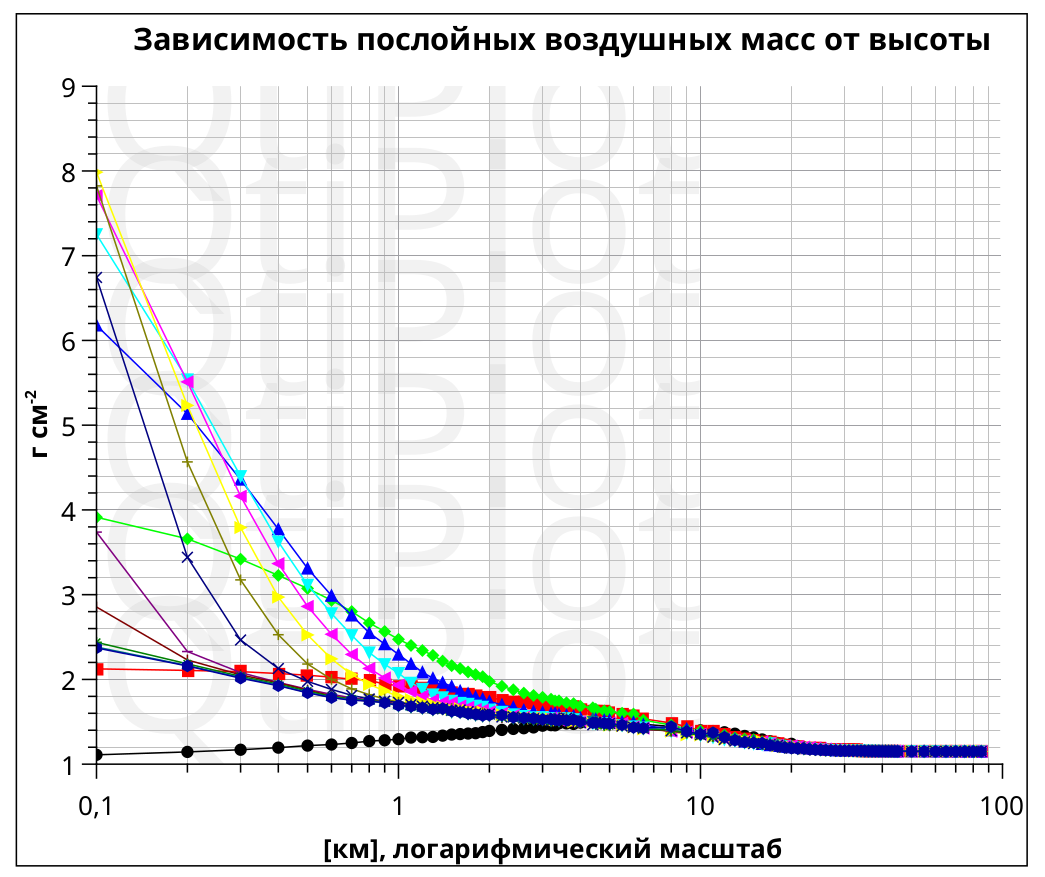
\includegraphics[width=\textwidth]{../experimental_data/2022-12-11_11-18.png}
    \textbf{Рис.1}
\end{minipage}
\begin{minipage}[b]{0.45\textwidth}
    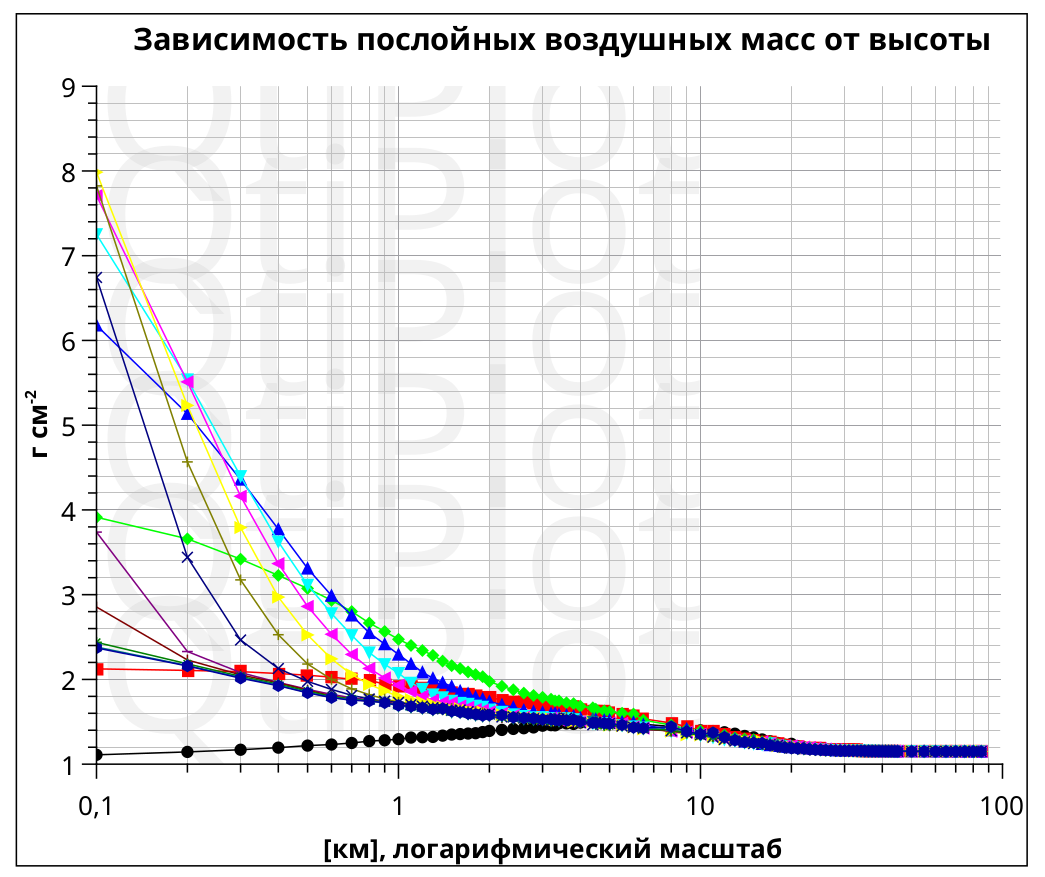
\includegraphics[width=\textwidth]{../experimental_data/2022-12-11_11-18.png}
    Рис.2
\end{minipage}
\end{figure}
\end{document} % конец документа




